% Chapter 4
\chapter{Transmission Expansion Planning by Quantum Annealing} % Main chapter title
\label{Chapter4} % For referencing the chapter elsewhere, use \ref{Chapter1} 
\section{Statement of the problem}
\begin{wrapfigure}{l}{0.35\textwidth}
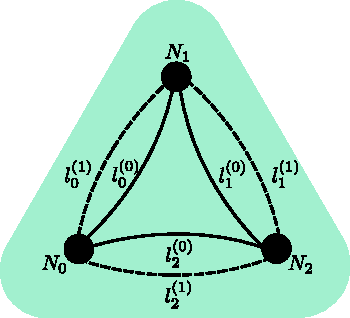
\includegraphics[scale=0.9]{Figures/3Node_Layer 1.pdf} 
\caption{An example considering a three node transmission expansion planning (TEP) problem with three candidate lines. Solid lines represent existing lines (super-index $(0)$) and dash lines are the candidate lines (super-index $(1)$).}
\label{fig:3node}
\end{wrapfigure}
\textit{Transmission expansion planning} (TEP)\cite{Neumann2020TransmissionFlows} is a mix integer linear problem (MILP) that aims at finding the optimal way to expand the capacity of an energy system. It decides how many components to build in order to satisfy the energy demand on a distributed energy system with a high share of renewable energy sources. The TEP scales badly using classical algorithms and, at the same time, energy system models are getting larger and more complex due to the integration of decentralized weather-dependent renewable energy sources, sector coupling and the increase of storage components. Currently, the problem is often linearized or the scope and granularity of the model are reduced using clustering algorithms. For this reason, any computational time reduction will have substantial implications in closing the granularity gap between what the current models can solve and the desired resolution needed by energy system operators.
Often these problems of improving the existing network to fulfill future targets are taken into account together under the name transmission expansion planning but in this case we are just considering transmission lines which allow us to reduce drastically the number of variables involve, so we can solve the problem with a quantum annealer, but at the same time the problem is not realistic. \par
We plan to scale the problem by increasing the number of nodes, targets to fulfill and the candidate components to build such as storage or generators of different carriers (wind turbines, heat pump, solar panels and so on). With the current state of quantum annealer such problems are not solvable with a pure quantum annealer. We required of hybrid quantum-classical methods to tackle out efficiently the problem.
\newpage
\begin{wraptable}{R}{7.2cm}
\centering
\begin{tabular}{cc} \\\toprule 
 \textbf{Symbol} & \textbf{Description} \\\midrule
 $\mathcal{N}$ & Nodes  \\\midrule
 $\mathcal{L}^{(0)}$ & Existing transmission lines  \\\midrule
 $\mathcal{L}^{(1)}$ & Candidate transmission lines \\\midrule
 $\mathcal{D}_{i}$ & Demand of node $i$. \\\midrule
 $\mathcal{G}_{i}$ & Energy generation at node $i$. \\\midrule
 $\mathcal{C}_{i}$ & Investment cost of line $i$ \\\bottomrule 
\end{tabular}
\caption{Nomenclature.}
\label{table:TEPNomenclature}
\end{wraptable}
We start by considering a small network of three nodes $N_{i}\in \mathcal{N}$ with 3 existing lines $l_{i}^{(0)}\in \mathcal{L}^{(0)}$ and 3 candidate lines $l_{i}^{(1)}\in \mathcal{L}^{(1)}$, (Figure \ref{fig:3node}). The nodes can be though as towns whose energy demand has to be fulfilled and the lines allow the network to transmit energy between nodes so that if some node is producing more energy than its demand, then that excess of energy can be transmitted to other node of the network. For now we are going to focus on the ability of each node in transmitting energy to other node assuming a set of snapshots is given, i.e., in each snapshot a node will require energy from the other two nodes. Our task is to fulfill this energy transmission demand between nodes so that our investment cost is minimum.
%%%%%%%%%%
\section{QUBO formulation of three-node TEP}
The objective function of TEP is
\begin{equation}
    \min_{s}\sum_{i=0}^{2}\mathcal{C}_{i}l_{i}^{(1)}
\end{equation}
subject to,
\begin{align}
    \mathcal{D}_{j} = \sum_{i=0}^{2}l_{i}^{(0)}, \quad \forall j \in \left[0,1,2\right] \\
    a
\end{align}
\section{Running QUBO problem on D-WAVE's annealer}

